%
% einleitung.tex -- Beispiel-File für die Einleitung
%
% (c) 2020 Prof Dr Andreas Müller, Hochschule Rapperswil
%
% !TEX root = ../../buch.tex
% !TEX encoding = UTF-8
%
\subsection{Zylinder\label{geodaeten:section:Standardverfahren:Zylinder}}
\rhead{Standardverfahren Beispiele}

Für die Zylinderoberfläche mit konstantem $r$ und dem metrischen Tensor 
\begin{equation}
	g_{ij} = \begin{pmatrix} 
		r^2 & 0 \\ 
		0 & 1 
	\end{pmatrix}
\end{equation}
wollen wir die Christoffel-Symbol berechnen. 
Wie bei dem kartesischen Raum (Abschnitt \ref{geodaeten:section:Standardverfahren:Kartesisch}) werden alle Christoffel-Symbol Null, da der metrische Tensor konstant ist\footnote{
Auch in diesem Beispiel sind die Christoffel-Symbol gleich Null.
Auf den ersten Blick könnte das verwirrend sein, da man bei einem Zylinder doch eindeutig eine Krümmung sieht.
Der Grund dafür ist, dass es sich bei dem Zylinder um eine extrinsische Krümmung handelt.
Die Zylinderoberfläche wird von aussen zu einem Zylinder gekrümmt.
Abgerollt sieht man allerdings, dass die Oberfläche flach ist.
Als weiteres Beispiel lässt sich berechnen, dass die Christoffel-Symbol im Polarkoordinaten-Raum nicht gleich Null sind und daher eine Krümmung existiert, obwohl der Raum flach erscheint.
Damit zeigt sich, dass die Intuition in diesem Fall täuschen kann.
}.
Wir ersparen uns hier deshalb diese Rechnung.

Setzt man $u^1 = \phi (t)$ und $u^2 = z(t)$ in die Geodätengleichung ein, so erhält man analog zu \eqref{geodaeten:equation:Standardverfahren:Kartesisch:x}
\begin{equation}
	\ddot{\phi}(t) = 0
	\label{geodaeten:equation:Standardverfahren:Zylinder:phi}
\end{equation}
und dementsprechend gemäss \eqref{geodaeten:equation:Standardverfahren:Kartesisch:y}
\begin{equation}
	\ddot{z}(t) = 0 .
\end{equation}


Wählen wir $P_A(\phi_1 , z_1) = P_A(1 , 1)$ und $P_B(\phi_2 , z_2) = P_B(3 , 5)$ gleich wie in Abschnitt \ref{geodaeten:section:Standardverfahren:Kartesisch}, kennen wie bereits die Lösungen. 
Aus \eqref{geodaeten:equation:StaKartesisch:LoesungX} wird 
\begin{equation}
	\phi(t) = 2t + 1 ,
\end{equation}
und aus \eqref{geodaeten:equation:StaKartesisch:LoesungY} wird
\begin{equation}
	z(t) = 4t + 1 .
\end{equation}

Beim Zylinder ist jedoch interessant, dass es beliebig viele weitere Lösungen für die Geodätengleichung gibt, da Die Winkelkoordinate periodisch ist.
Durch Hinzufügen eines Vielfachen von $2\pi$ macht die Kurve zusätzliche Runden um den Zylinder, bevor sie auf den Punkt $P_B$ trifft, wie in Abbildung \ref{geodaeten:figure:Standardverfahren:Zylinder:figure1} dargestellt.
Dies ist zwar nicht die kürzeste Strecke, jedoch wird weder die Gleichung \eqref{geodaeten:equation:Standardverfahren:Zylinder:phi} verletzt noch der Punkt $P_A$ oder $P_B$ verfehlt.
Deshalb existieren sie als Scheinlösungen der Geodätengleichung.

Wird die Oberfläche des Zylinders wie in Abbildung \ref{geodaeten:figure:Standardverfahren:Zylinder:figure1} auf eine Fläche abgerollt, ist ersichtlich, wie auch hier der kürzeste Weg eine Gerade ist.  

\begin{figure}
	\centering
	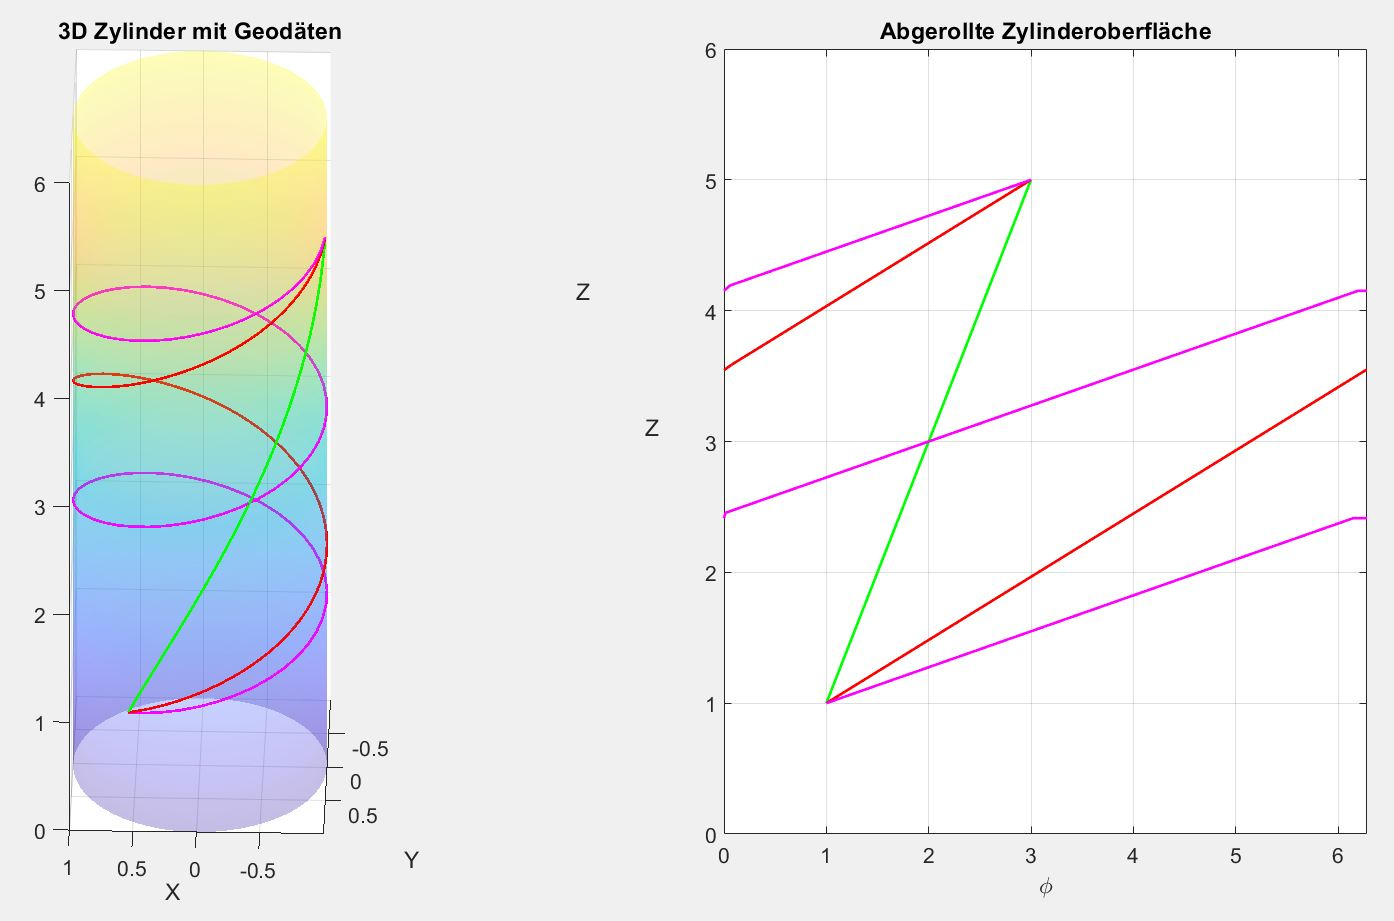
\includegraphics[width=\textwidth]{papers/geodaeten/Abbildungen/Standardverfahren/Zylinder}
	\caption{Darstellung der Geodätenlinien auf einem Zylinder und dessen abgerollte Oberfläche in einem 2D Plot mit Matlab.}
	\label{geodaeten:figure:Standardverfahren:Zylinder:figure1}
\end{figure}
